\documentclass{article}
\usepackage[utf8]{inputenc}
\usepackage[english]{babel}

\title{Asymptotic Notation}
\author{Manuel Serna-Aguilera}
\date{}

\usepackage{natbib}
\usepackage{graphicx}
\usepackage{amsmath}

% The command \newtheorem{theorem}{Theorem} has two parameters, the first one is the name of the environment that is defined, the second one is the word that will be printed, in boldface font, at the beginning of the environment. Once this new environment is defined it can be used normally within the document, delimited it with the marks \begin{theorem} and \end{theorem}.
\newtheorem{theorem}{Theorem}

\begin{document}

\maketitle
Asymptotic notation is used by the book to describe the running times of algorithms. By asymptotic efficiency, the book means we should be concerned only with an input size large enough that we will only care about the order of the growth of the running time (like $n$, $n^2$, ...). Thus, we look at how the running time increases with the size of the input. Asymptotic notation applies to \textit{functions}, and recall these functions are the summations of all lines within the procedure and how often these lines run. 
\\ \\
For example, a running time $an^2 + bn + c$ is dominated by the leading term $n^2$, thus this running time (like insertion sort's worst-case running time) can be written as $\Theta{(n^2)}$, and this can characterize the best-case, average-case, or as it is often the case, worst-case running times.

\begin{figure}[ht]
\centering
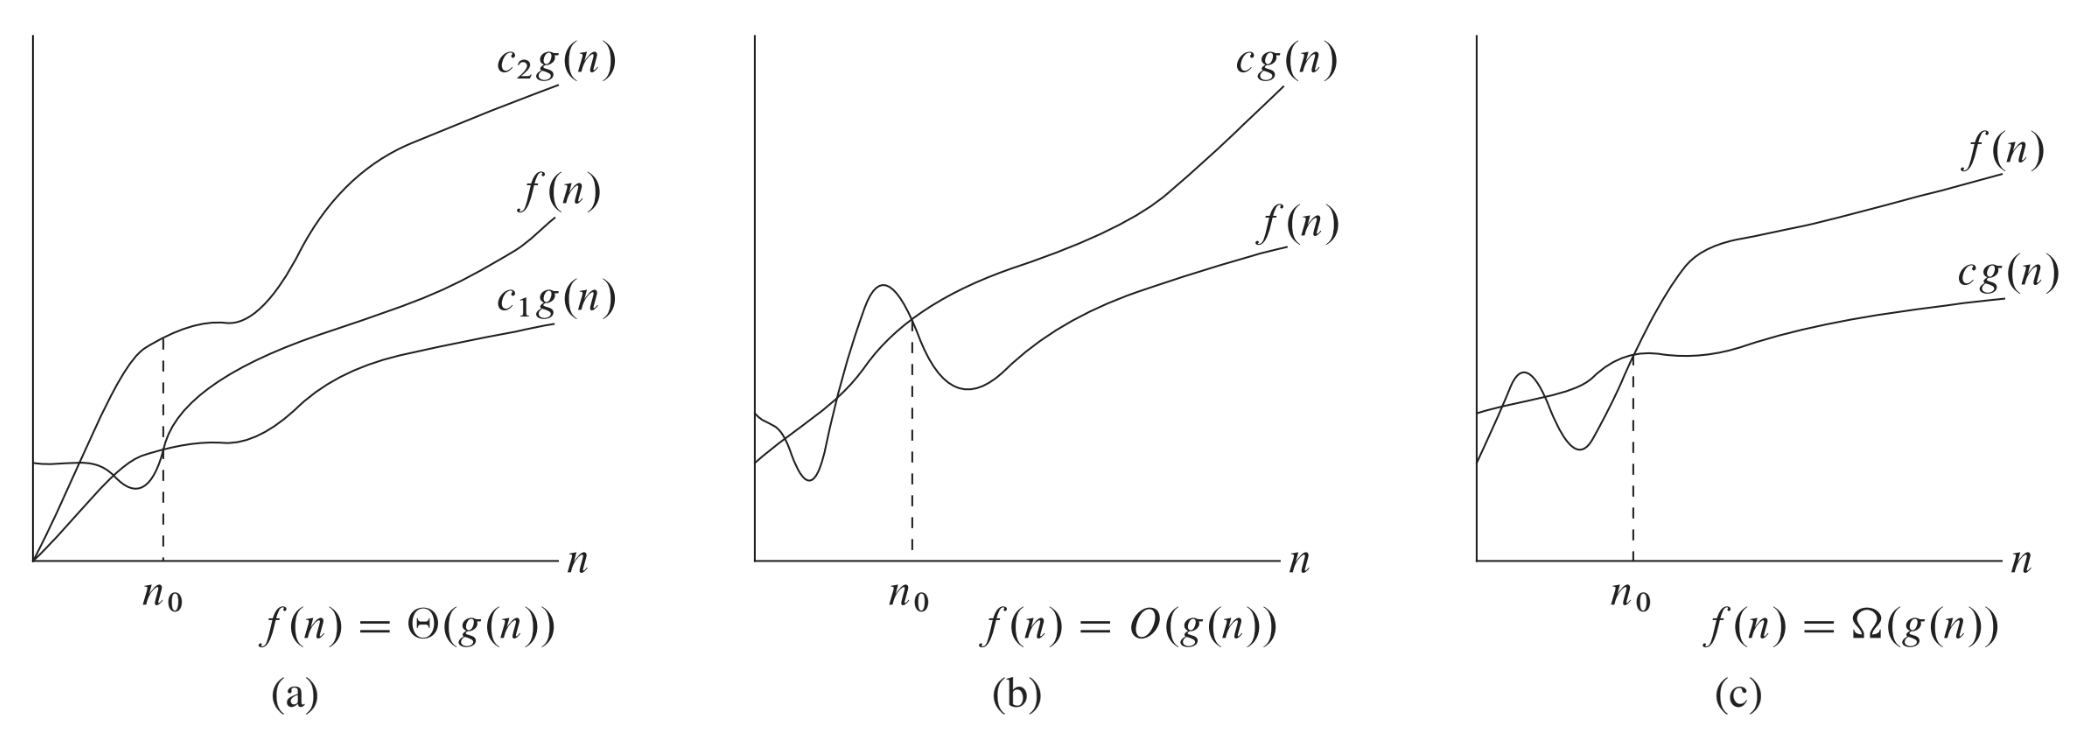
\includegraphics[scale=0.35]{asymptotic_notation}
\caption{
    Graphic examples of $\Theta$ $O$, and $\Omega$ notations. The value $n_0$ is the minimum value for the asymptotic notation to apply.
    \textbf{(a)} $\Theta$-notation bounds a function to within constant factors. We write $f(n)=\Theta{(g(n))}$ if there exist positive constants $n_0$, $c_1$, and $c_2$ such that at and to the right of $n_0$, the value of $f(n)$ always lies between $c_1g(n)$ and $c_2g(n)$ inclusive.
    \textbf{(b)} $O$-notation gives an \textit{upper} bound for a function to a constant factor. $f(n)$ will be between 0 and $cg(n)$ inclusive.
    \textbf{(c)} $\Omega$-notation gives a \textit{lower} bound for a function to within a constant factor. $f(n)$ will be between two of $cg(n)$ on the bottom and is essentially not bounded going up. We do want to limit growth in this direction, however.
}
\label{fig:asymptotic_notation}
\end{figure}

\newpage

The book interprets the equal sign in this context as $f(n)$ belonging to a set of functions $\_\_\_(g(n))$ (fill in the blank with whatever notation). Therefore $f(n)=\_\_\_(g(n))$ is the same as $f(n) \in \_\_\_(g(n))$. The reason the book utilizes $=$ instead of $\in$ is to relate running times/costs (derived by looking at costs for each line, for example) with a generalized running time.
\\ \\
This makes sense as functions grow slower, faster, or at the same rate as what you're comparing them to, your $g(n)$. For all $n \geq n_0$, the function $f(n)$ is equal to $g(n)$ to within a \textit{constant factor}, we say that $g(n)$ is an \textbf{asymptotically tight bound} for $f(n)$. Another term the book uses is \textbf{asymptotically nonnegative}; an \textbf{asymptotically nonnegative} function is one that is positive for all sufficiently large n. As a consequence, the function $g(n)$ itself must be asymptotically nonnegative, or the set \_\_\_$(g(n))$ must be empty. 

\newpage

%================================================
\section*{$\Theta$-notation}
%================================================
For a given function $g(n)$, we denote by $\Theta{(g(n))}$ the \textit{set of functions}\newline
\begin{equation*}
\begin{split}
\Theta{(g(n))} = \{f(n) & : \text{there exist positive constants } c_1, c_2, \text{ and } n_0 \text{ such that}\\
  & 0 \leq c_1g(n) \leq f(n) \leq c_2g(n) \text{ for all } n \geq n_0\}.
\end{split}
\end{equation*}
For sufficiently large $n$, the function $f(n)$ is "sandwiched" between $c_1g(n)$ and $c_2g(n)$.

%================================================
\section*{$O$-notation}
%================================================
$O$-notation asymptotically bounds a function from above and below. $O$-notation is used when there is only a asymptotic upper bound, the lower bound is just zero. \newline
For a given function $g(n)$, we denote by $O{(g(n))}$ the set of functions\newline
\begin{equation*}
\begin{split}
O{(g(n))} = \{f(n) & : \text{there exist positive constants } c\text{ and } n_0 \text{ such that}\\
  & 0 \leq f(n) \leq cg(n) \text{ for all } n \geq n_0\}.
\end{split}
\end{equation*}
\textbf{\emph{Important}}: $f(n)=\Theta{(g(n))}$ implies $f(n)=O{(g(n))}$, as $\Theta$-notation is a stronger notation than $O$-notation. The use of this set notation only says there is an asymptotic upper bound, this notation says nothing about how tight the upper bound is (the lower bound is tight since it is zero).

%================================================
\section*{$\Omega$-notation}
%================================================
$\Omega$-notation provides an \textbf{asymptotic lower bound}.\newline
For a given function $g(n)$, we denote by $\Omega$ the set of functions\newline
\begin{equation*}
\begin{split}
\Omega{(g(n))} = \{f(n) & : \text{there exist positive constants } c\text{ and } n_0 \text{ such that}\\
  & 0 \leq cg(n) \leq f(n) \text{ for all } n \geq n_0\}.
\end{split}
\end{equation*}

\begin{theorem}
For any two functions f(n) and g(n), we have f(n) = $\Theta{(g(n))}$ if and only if f(n) = O(g(n)) and f(n) = $\Omega{(g(n))}$.
\end{theorem}

\newpage

%================================================
\section*{$o$-notation}
%================================================
The asymptotic upper bound provided by $O$-notation may or not be asymptotically tight, as the book notes. The bound $2n^2=O(n^2)$ is asymptotically tight, but the bound $2n=O(n^2)$ is not. All $o$-notation says is a bound is $\textbf{not}$ asymptotically tight.\newline
We formally define $o(g(n))$ as the set
\begin{equation*}
\begin{split}
o{(g(n))} = \{f(n) & : \text{for any positive constant } c > 0,\text{ there exists a constant}\\
  & n_0 > 0 \text{ such that } 0 \leq f(n) < cg(n) \text{ for all } n \geq n_0\}.
\end{split}
\end{equation*}
The main difference between $O$-notation and $o$-notation is that in $f(n)=O(g(n))$, the bound $0 \leq f(n) \leq cg(n)$ holds for \textit{some} constant $c > 0$, but in $f(n)=o(g(n))$, the bound $0 \leq f(n) < cg(n)$ holds for \textit{all} constants $c > 0$ (notice the $>$ used for $o$-notation).
\\ \\
The function $f(n)$ becomes insignificant relative to $g(n)$ as $n$ approaches infinity, that is,
\newline
$$\lim_{n\to\infty} \frac{f(n)}{g(n)} = 0.$$

%================================================
\section*{$\omega$-notation}
%================================================
$\omega$-notation is to $\Omega$-notation as $o$-notation is to $O$-notation. $\omega$-notation is used to denote a lower-bound that is \textbf{not} asymptotically tight.\\
Formally, however, $\omega(g(n))$ is the defined to be the set\newline
\begin{equation*}
\begin{split}
\omega{(g(n))} = \{f(n) & : \text{for any positive constant } c > 0,\text{ there exists a constant}\\
  & n_0 > 0 \text{ such that } 0 \leq cg(n) < f(n) \text{ for all } n \geq n_0\}.
\end{split}
\end{equation*}
For example, $n^2/2 = \omega{(n)}$, but $n^2/2 \neq \omega{(n^2)}$. The relation $f(n) = \omega{(g(n))}$ implies that\newline
$$\lim_{n\to\infty} \frac{f(n)}{g(n)} = \infty,$$
if the limit exists. That is, $f(n)$ becomes arbitrarily large relative to $g(n)$ as $n$ increases to infinity.

\newpage

%================================================
\section*{More Information}
%================================================
For the following, assume that $f(n)$ and $g(n)$ are asymptotically positive.
\\ \\
\textbf{Transitivity:}\\
\begin{equation*}
f(n) = \Theta{(g(n))} \text{ and } g(n) = \Theta{(h(n))} \text{ imply } f(n) = \Theta{(h(n))}
\end{equation*}
\begin{equation*}
f(n) = O{(g(n))} \text{ and } g(n) = O{(h(n))} \text{ imply } f(n) = O{(h(n))}
\end{equation*}
\begin{equation*}
f(n) = \Omega{(g(n))} \text{ and } g(n) = \Omega{(h(n))} \text{ imply } f(n) = \Omega{(h(n))}
\end{equation*}
\begin{equation*}
f(n) = o{(g(n))} \text{ and } g(n) = o{(h(n))} \text{ imply } f(n) = o{(h(n))}
\end{equation*}
\begin{equation*}
f(n) = \omega{(g(n))} \text{ and } g(n) = \omega{(h(n))} \text{ imply } f(n) = \omega{(h(n))}
\end{equation*}
\\
\textbf{Reflexivity:}\\
\begin{equation*}
f(n) = \Theta{(f(n))}
\end{equation*}
\begin{equation*}
f(n) = O{(f(n))}
\end{equation*}
\begin{equation*}
f(n) = \Omega{(f(n))}
\end{equation*}
\\ \\
\textbf{Symmetry:}
\\ \\
$f(n) = \Theta{(g(n))}$ if and only if $g(n) = \Theta{(f(n))}$
\\ \\
\textbf{Transpose Symmetry:}\\
\begin{equation*}
f(n) = O{(g(n))} \text{ if and only if } g(n) = \Omega{(f(n))}
\end{equation*}
\begin{equation*}
f(n) = o{(g(n))} \text{ if and only if } g(n) = \omega{(f(n))}
\end{equation*}
Because these properties hold for asymptotic notations, we can draw an analogy between the asymptotic comparison of two functions $f$ and $g$ and the comparison of two real numbers $a$ and $b$:
\begin{equation*}
f(n) = O{(g(n))} \text{ is like } a \leq b
\end{equation*}
\begin{equation*}
f(n) = \Omega{(g(n))} \text{ is like } a \geq b
\end{equation*}
\begin{equation*}
f(n) = \Theta{(g(n))} \text{ is like } a = b
\end{equation*}
\begin{equation*}
f(n) = o{(g(n))} \text{ is like } a < b
\end{equation*}
\begin{equation*}
f(n) = \omega{(g(n))} \text{ is like } a > b
\end{equation*}
We say that $f(n)$ is \textbf{asymptotically smaller} than $g(n)$ if $f(n) = o(g(n))$, and $f(n)$ is \textbf{asymptotically larger} than $g(n)$ if $f(n) = \omega{((g(n)))}$.

\newpage

%================================================
\section*{Monotonicity}
%================================================
A function $f(n)$ is \textbf{monotonically increasing} if $m \leq n$ implies $f(m) \leq f(n)$. Similarly, it is \textbf{monotonically decreasing if $m \leq n$} implies $f(m) \geq f(n)$. A function $f(n)$ is \textbf{strictly increasing} if $m < n$ implies $f(m) < f(n)$ and \textbf{strictly decreasing} if $m < n$ implies $f(m) > f(n)$
\\ \\
Also look at chapter 3 section 2 for more information on common functions. It would also be a good idea to look at the appendices at the back of the book, as they offer relevant mathematical background that will prove useful when dealing with the rest of the material of the book.

\end{document}
